\chapter{Discussion \& Conclusions}

\section{Complexity}

When the network grow it will eventually become to cumbersome for every node to Floyd-Warshall the whole network as this simulation assumes. Approx. will probably be used. Ant routing tables have been suggested but might be problem with lying about connectedness.

\section{Balanced Channels}

At first sight it may seem obvious that the fee price structure is flawed as it cannot incentive, e.g give a discount, for a route in such a direction so it leaves channels in a more balanced state. A change in fee structure obviously change the validity of each strategy.

Suppose there exists a channel between Alice and Bob with 10 million satoshis in it. 
Two payments, $P_{1}$ and $P_{2}$ are routed through the channel from Bob to Alice.
Both use the same amount of liquidity, 3,500,000 satoshis each, but they start from two different initial states $B_{1}$ and $B_3$.

\begin{figure}[!htb]
	\hspace*{0.7cm} 
	\centering
	\includegraphics[width=7cm]{images/protocol_upgrade.png}
	
	\label{fig:xt_nodes}
	\hspace*{2mm} 	
\end{figure}

The two payments would incur the same fee, 

\[ F_{P_1 P_2} = F_B + (3,500,000 * F_R / 1,000,000) \]

but leave the channels in completely different states. $P_1$ at $B_2$ and $P_2$ at $B_4$. It is of course possible to bump the channel price after $P_1$ to
be more expensive, but suppose a third larger payment $P_3$ going from $B_1$ to $B_4$ would still run into this problem.

If a naive structure, that takes the state, is considered so as the issues of such a solution arise. 

Each satoshi in the channel could be seen as a different bracket, with a different price for each satoshi moved. The channels would then broadcast a cost function instead of the fixed fee.

\begin{figure}[!htb]
	\hspace*{-0.5cm}
	\centering
	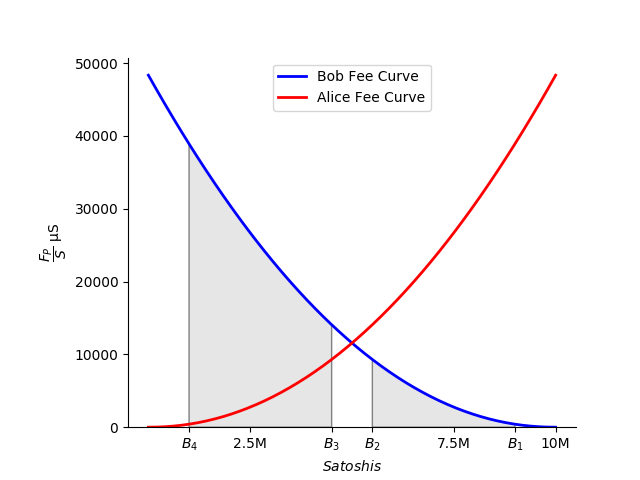
\includegraphics[width=9cm]{images/fee_scheme.png}
	\label{fig:xt_nodes}
	\hspace{2mm}
\end{figure}

From the cost function the fee may be retrieved by calculating the area under the graphs. Some deterministic way to round the fee to whole satoshis and some way to verify the function is formulated correctly must be defined. 

The fees for $P_1$, $P_2$ would be very different with this brackets method.

\[ F_{P_1} = F_{B} + \int_{B_1}^{B_2} f(x) dx = F_B + 13,502,153,930 \mu S \] 

\[ F_{P_2} = F_{B} + \int_{B_3}^{B_4} f(x) dx  = F_B + 88,984,850,361 \mu S \]

Here the fees are much larger for the payment that unbalances the channel than the payment that balances it. 

However there are some clear problems with this approach. Every new payment would require each node on the path to rebroadcast the new balance to all other nodes\footnote{As brought up by Andrea Rapitzu.~\cite{raspitzu:fee}}. Which would scale even worse than the Bitcoin bottom layer in message passing. There would also be privacy issues as any observant node could track the payments through balance updates\footnote{As brought up by ZmnSCPxj.~\cite{ZmnSCPxj:fee}}.

It is further unclear how much immediate balance will matter for routing success and other solutions have been proposed to levitate this pressure point. E.g René Pickhardt JIT-routing~\cite{pickard:jit} and branching out utilizing multiple paths to fulfill liquidity needs.   


\section{Future work}

As 